\section{Pressure from flow MRI}
\label{sec:mri}
The inverse setting of the wake problem is the one that matters clinically: 4D flow MRI~\cite{markl2012} measures
the velocity of blood in three dimensions over the heartbeat, but not its pressure, and the pressure drop across an
aortic coarctation is still measured with a catheter or estimated with the simplified Bernoulli rule
$\Delta p=4v_{\max}^2$ (mmHg, m/s), which ignores friction, unsteadiness and the jet's shape. A network trained on the
measured velocity and on \eqref{eq:rm} returns a pressure field that no instrument recorded~\cite{kissas2020}. We
tested this first on a synthetic stenosis with a known answer and then on a public phantom with catheter pressure.

\paragraph{Synthetic stenosis.} A 6~mm channel with a 60\% narrowing at $\Rey=150$ (and a faster jet, 70\% at
$\Rey=300$) was solved with a projection method at 50 cells per diameter; the ``scan'' averages that flow over
0.6~mm voxels and 24 phases and adds noise at an SNR of 20. Only the scan enters the loss, as voxel- and
phase-averaged data. With the walls as soft loss terms the network learned almost no pressure ($7\times10^{-4}$~mmHg
against 0.59): the walls slipped and the flow needed no pressure gradient. Building the walls into a stream function,
$\psi=Q(t)\,f(\eta)$ with $\eta=y/h(x)$ and a learnt Fourier flow rate $Q(t)$, gave peak drops of 0.557~mmHg against
0.594 (6.2\%) and 3.96 against 4.13 (4.1\%), and the hidden pressure field to 3.9\% and 9.0\%; Bernoulli applied to
the same scans is 31\% and 21\% too high. L-BFGS on one fixed batch fitted the noise (loss $1.6\to1.4\times10^{-4}$)
and doubled the pressure error, so the Adam result is used.

\paragraph{Phantom and baselines.} The 4D-FlowP dataset~\cite{nair4dflowp} contains eight 3D-printed aortic
coarctations (two patient geometries, baseline and severe narrowing, normal and low flow) in a pulsatile loop with a
glycerol--water fluid, scanned with 4D flow MRI (1.8~mm, 60~ms), an acceleration-encoded acquisition, and catheter
pressure in the ascending (AAo) and descending aorta (DAo) at 1~kHz. Preparation corrects eddy-current offsets with a
second-order fit on static voxels, segments the lumen by speed, recovers the sign of each velocity component by
minimising the divergence of the measured flow, and aligns the catheter's beat with the scan's by cross-correlating
the flow-meter waveform with the scan's flux (offsets of 121--147~ms, correlation 0.97--1.00). Computed from the same
scans, Bernoulli has a mean peak-drop error of 30.4\% against the catheter and a pressure Poisson
estimate 45.7\% (Table~\ref{tab:phantom}); both are low on every case.

\paragraph{Network and development.} The velocity network is the gated MLP of Section~\ref{sec:method}, periodic over
the beat, trained on voxel-averaged data (four sub-samples per voxel) with residual- and misfit-based resampling. On
the development case (P2 baseline, catheter 13.1~mmHg) a network with a shared pressure output fitted the flow (peak
jet 9\% slow) but predicted 0.30~mmHg. A path integral of \eqref{eq:rm} along a 259~mm centreline showed that the
network's own velocity required 4.5--6.2~mmHg during systole: the network had placed the flow's acceleration in a
small, coherent momentum residual (about 0.02 per unit length, invisible in a mean-square loss) instead of in
$\nabla p$. A pressure fitted to the frozen velocity alone gave 7.26~mmHg with a third less residual and followed the
catheter waveform with correlation 0.96. A separate pressure network with 12 harmonics of the beat raised the joint
result to 5.3~mmHg at the same budget. A learnt eddy-viscosity field collapsed to zero within 20k steps whatever its
penalty, because the data can be fitted without it; a Smagorinsky viscosity~\cite{smagorinsky1963} with $C_s=0.17$,
computed from the resolved flow, stayed near the molecular value. With the measured acceleration added as a data term
the drop reached 8.74~mmHg after 60k steps (33.3\% error; Bernoulli 39\% and pressure Poisson 40\% on this case). The
scan's jet peaks at 1.42~m/s, while 13.1~mmHg corresponds to about 1.8~m/s, so the remaining gap is in the data.

\begin{table*}[t]
\centering
\caption{Peak pressure drop (mmHg) on the eight phantom cases, design frozen after P2 baseline; error against the
catheter in brackets. PINN: laminar pressure network, and Smagorinsky viscosity with the measured acceleration (60k
steps each). Last row: networks read at the catheter's own marker positions instead of the 2D phase-contrast planes.}
\label{tab:phantom}
\small
\begin{tabular}{@{}lccccc@{}}
\toprule
case & catheter & Bernoulli & pressure Poisson & PINN, laminar & PINN, Smagorinsky + acceleration\\
\midrule
P1 baseline & 16.2 & 10.3 (36) & 6.5 (60) & 20.3 (25) & 22.1 (36)\\
P1 severe & 24.7 & 22.0 (11) & 10.2 (59) & 16.4 (33) & 16.3 (34)\\
P2 baseline$^{*}$ & 13.1 & 8.0 (39) & 7.9 (40) & 8.8 (33) & 8.7 (33)\\
P2 severe & 20.8 & 16.7 (20) & 14.5 (30) & 4.8 (77) & 3.7 (82)\\
P1 baseline, low flow & 8.9 & 5.1 (43) & 5.3 (41) & 14.8 (65) & 14.9 (67)\\
P1 severe, low flow & 13.4 & 12.0 (10) & 6.7 (50) & 9.8 (27) & 11.8 (12)\\
P2 baseline, low flow & 7.2 & 3.9 (46) & 4.9 (32) & 5.7 (21) & 6.4 (11)\\
P2 severe, low flow & 12.0 & 7.4 (38) & 5.5 (54) & 5.2 (57) & 4.7 (61)\\
\midrule
mean error & & 30.4\% & 45.7\% & 42.3\% & 42.0\%\\
mean error, read at the catheter markers & & & & 45.5\% & 43.5\%\\
\bottomrule
\multicolumn{6}{@{}l@{}}{\footnotesize $^{*}$Development case; the other seven are held out.}
\end{tabular}
\end{table*}

\begin{figure}[t]
\centering
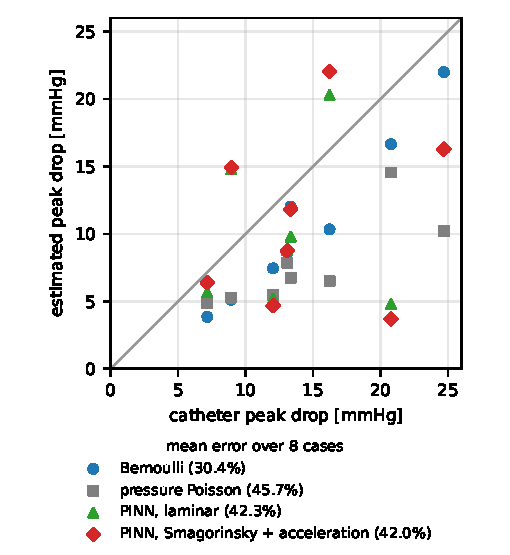
\includegraphics[width=0.85\columnwidth]{figures/phantom_cases.pdf}
\caption{Peak drop of every method against the catheter on the eight phantom cases.}
\label{fig:phantom}
\end{figure}

\paragraph{Held-out test.} Frozen after the development case and run unchanged on all eight
(Table~\ref{tab:phantom}, Fig.~\ref{fig:phantom}), the networks reach a mean error of 42.3\% (laminar) and 42.0\% (with
acceleration), behind Bernoulli and ahead of the pressure Poisson estimate; over the seven held-out cases alone 43.6\%
and 43.3\%. The gate, a lower mean error than Bernoulli, is missed. The slope against the catheter is about 0.7 but
$R^2$ is negative, so the errors are not a correctable bias. The acceleration helps where it registers well onto the
velocity scan (P2 baseline at low flow $21\to11\%$, P1 severe at low flow $27\to12\%$) and hurts where it does not
(P2 severe, Dice 0.65, $77\to82\%$). The networks fail in two ways: far too low on the severe P2 jets and far too
high on the P1 baseline cases with or without the acceleration.

The second failure is partly one of evaluation. The catheter recorded the DAo at five positions, between which its
drop changes by a factor of two on geometry P1 (P1 baseline 11.7--23.2~mmHg; within 1.4~mmHg on P2), and the
networks' drop rises steadily down the descending aorta (13.7 to 30.8~mmHg on P1 baseline). We located the gel
markers of the catheter positions in each case's 1~mm anatomy scan and re-read the trained networks, without
retraining, as cross-section means at the AAo marker and the middle DAo marker. P1 baseline then drops to 7--9\%, but
every other case gets worse, since the phase-contrast outlet plane lay near the lowest marker: the mean becomes
43.5\% (acceleration) and 45.5\% (laminar). The severe narrowings fail most, at 2--4~mmHg against 12--21: a narrow,
fast jet is what voxel and phase averaging remove, and the equations cannot restore a velocity peak that is absent
from the data they are fitted to.
